\documentclass[aspectratio=169, usenames,svgnames,dvipsnames]{beamer}
\usepackage[utf8]{inputenc}
\usepackage[T1]{fontenc}
\usepackage{graphicx}
\usepackage{cancel}
\usepackage{grffile}
\usepackage{longtable}
\usepackage{tikz}
\usepackage{changepage}
\usepackage{wrapfig}
\usepackage{rotating}
\usepackage[normalem]{ulem}
\usepackage[spanish]{babel} % para decimales con coma en lugar de punto
\usepackage{amsmath}
\usepackage{textcomp}
\usepackage{amssymb}
\usepackage{capt-of}
\usepackage{hyperref}
\usepackage{color}
\usepackage{listings}
\usepackage{mathpazo}
\usepackage{gensymb}
\usepackage{amsmath}
\usepackage{diffcoeff}
\usepackage{steinmetz}
\usepackage{mathtools}
\usepackage{xparse} % For "overbrace/underbrace but with an arrow instead", from https://tex.stackexchange.com/questions/8720/overbrace-underbrace-but-with-an-arrow-instead
\usepackage{minibox} % Para poder partir el texto en 2 líneas usando "underbrace" u "overbrace", info aquí: https://tex.stackexchange.com/questions/8680/how-can-i-insert-a-newline-in-a-framebox
\bibliographystyle{plain}
\usepackage{siunitx}
\sisetup{output-decimal-marker={,}, retain-unity-mantissa = false}
\DeclareSIUnit{\watthour}{Wh}
\DeclareSIUnit\var{VAr}
\hypersetup{colorlinks=true, linkcolor=Blue, urlcolor=Blue}
\renewcommand{\thefootnote}{\fnsymbol{footnote}}
\newcommand{\laplace}[1]{\mathbf{#1}(\mathbf{s})}
\newcommand{\slp}{\mathbf{s}}
\newcommand{\fasor}[1]{\mathbf{#1}(\omega)}
\newcommand{\atan}{\mathrm{atan}}
\parskip=5pt
\usetheme{Boadilla}
\usecolortheme{rose}
\usefonttheme{serif}
\author{Autor: \hspace{2mm} Luis Badesa Bernardo}
\date{}
\title{Introducción al régimen transitorio \vspace{3mm}}
\subtitle{Teoría de Circuitos}
\setbeamercolor{alerted text}{fg=blue!50!black} \setbeamerfont{alerted text}{series=\bfseries}
\AtBeginSubsection[]{\begin{frame}[plain]\tableofcontents[currentsubsection,sectionstyle=show/shaded,subsectionstyle=show/shaded/hide]\end{frame}}
\AtBeginSection[]{\begin{frame}[plain]\tableofcontents[currentsection,hideallsubsections]\end{frame}}
\beamertemplatenavigationsymbolsempty
\setbeamertemplate{footline}[frame number]
\setbeamertemplate{itemize items}[triangle]
\setbeamertemplate{enumerate items}[circle]
\setbeamertemplate{section in toc}[circle]
\setbeamertemplate{subsection in toc}[circle]
\hypersetup{
 pdfauthor={Luis Badesa Bernardo},
 pdftitle={Introducción al régimen transitorio},
 pdfkeywords={},
 pdfsubject={},
 pdfcreator={}, 
 pdflang={Spanish}}

% Para poner flechas sobre los signos de igual, de aquí: https://tex.stackexchange.com/questions/8720/overbrace-underbrace-but-with-an-arrow-instead
\NewDocumentCommand{\overarrow}{O{=} O{\uparrow} m}{%
  \overset{\makebox[0pt]{\begin{tabular}{@{}c@{}}#3\\[0pt]\ensuremath{#2}\end{tabular}}}{#1}
}
\NewDocumentCommand{\underarrow}{O{=} O{\downarrow} m}{%
  \underset{\makebox[0pt]{\begin{tabular}{@{}c@{}}\ensuremath{#2}\\[0pt]#3\end{tabular}}}{#1}
}

% Para "footnotes" sin asterisco:
\newcommand\blfootnote[1]{%
    \begingroup
    \renewcommand\thefootnote{}\footnote{#1}%
    \addtocounter{footnote}{-1}%
    \endgroup
} % Sacado de https://tex.stackexchange.com/questions/30720/footnote-without-a-marker

 
\begin{document}

\maketitle

\section{Introducción}

\begin{frame}{¿Qué es el régimen transitorio?} 
    \vspace{3mm}
    \begin{itemize}
        \item Ejemplo: \alert{encendido} de circuito de \alert{continua} (con transitorio \textit{subamortiguado})
    \end{itemize}

    \vspace{-2mm}
    \begin{center}
        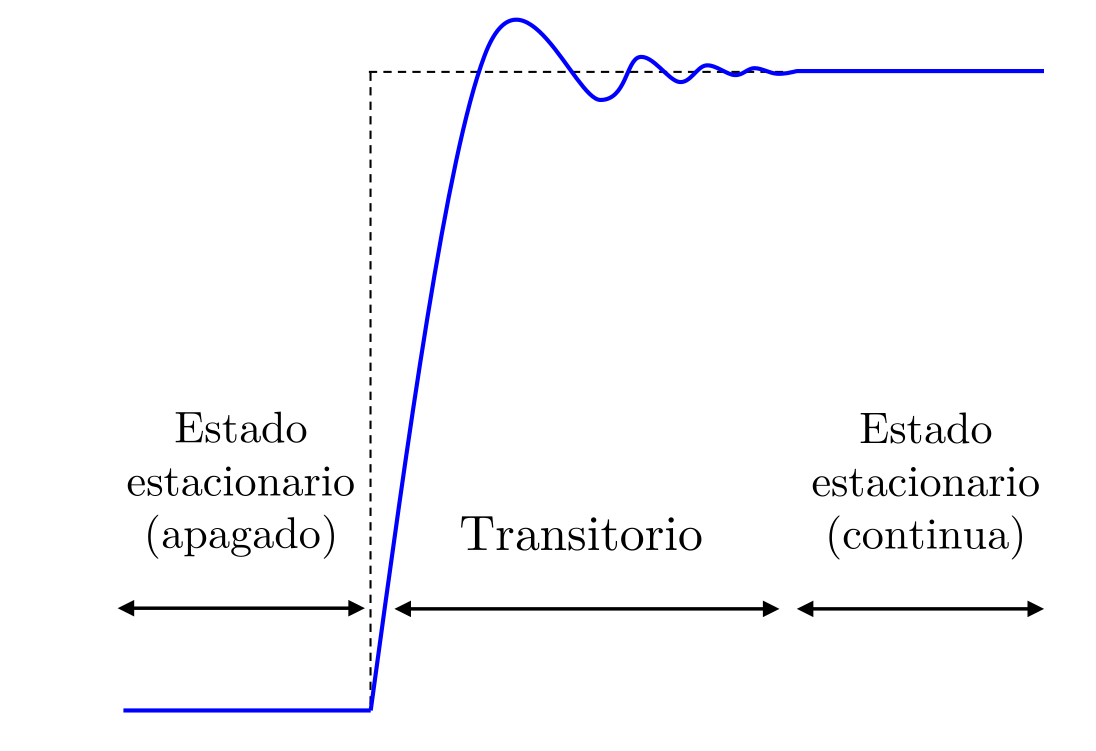
\includegraphics[height=0.8\textheight]{../figs/ej_transitorio_DC.pdf}
    \end{center}
\end{frame}

%%%%%%%%%%%%%%%%%

\begin{frame}{¿Qué es el régimen transitorio?} 
    \vspace{3mm}
    \begin{itemize}
        \item Ejemplo: \alert{aumento de voltaje} en circuito de \alert{alterna} (con transitorio \textit{sobreamortiguado})
    \end{itemize}

    \vspace{-2mm}
    \begin{center}
        \includegraphics[height=0.8\textheight]{../figs/ej_transitorio_AC.pdf}
    \end{center}
\end{frame}

%%%%%%%%%%%%%%%%%

\begin{frame}{Régimen transitorio \hspace{3mm}\textit{vs.}\hspace{3mm} estado estacionario}
    \vspace{4mm}
    
    \begin{block}{Estado estacionario o ``régimen permanente''}
        \begin{itemize}
            \vspace{1mm}
            \item Circuito \alert{estabilizado}
            
            \vspace{1mm}
            \item Las \alert{tensiones} y \alert{corrientes} de un circuito son \alert{constantes} (CC) o \alert{periódicas} (CA)

            \vspace{1mm}
            \item Modelado matemático: \alert{ecuaciones algebraicas}

            \vspace{1mm}
        \end{itemize}        
    \end{block}

    \vspace{2mm}
    \begin{block}{Régimen transitorio}
        \begin{itemize}
            %\vspace{1mm}
            %\item Para alcanzar el régimen permanente (o para alternar entre dos regímenes permanentes) el circuito atraviesa el régimen transitorio
            %
            \vspace{1mm}
            \item \alert{Cambio} en las \alert{condiciones} de funcionamiento de un \alert{circuito}: 

            \vspace{1mm}
            encendido o apagado de fuentes, o cambio en las cargas $\;\rightarrow\;$ \alert{interruptores}
            
            \vspace{1mm}
            \item Variación de ${\boldsymbol{\color{blue!50!black} u(t)}}$ e $\,{\boldsymbol{\color{blue!50!black} i(t)}}$ hasta alcanzar nuevos valores

            \vspace{1mm}
            \item Modelado matemático: \alert{ecuaciones diferenciales}

            \vspace{1mm}
        \end{itemize}
    \end{block}
\end{frame}

%%%%%%%%%%%%%%%%%

\begin{frame}{Acumulación de energía}
    \begin{block}{Estado estacionario}
        \begin{itemize}
            \vspace{1mm}
            \item \alert{Energía acumulada} en \alert{bobinas} y \alert{condensadores}
            
            \vspace{1mm}
        \end{itemize}
    \end{block}

    \vspace{4mm}
    \begin{block}{Régimen transitorio}
        \begin{itemize}
            \vspace{1mm}
            \item \alert{Redistribución} y \alert{disipación} de energía acumulada

            \vspace{1mm}
            \item La redistribución de energía \alert{no} es \alert{inmediata}

            \vspace{1mm}
            \alert{Duración corta} (\(\si{\micro\second}\)) pero superior a \qty{0}{\second}, dependiendo de \alert{relación entre} \alert{acumulación} y \alert{disipación} (resistencia)

            \vspace{1mm}
        \end{itemize}
    \end{block}
\end{frame}

%%%%%%%%%%%%%%%

\begin{frame}{Consigna habitual: \hspace{3mm}función escalón} \label{diapo:escalon}
    \begin{columns}
    \begin{column}{0.7\columnwidth}
        \begin{center}
            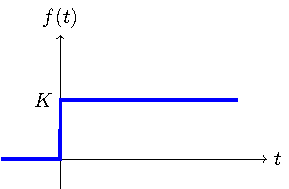
\includegraphics[width=.7\linewidth]{../figs/escalon.pdf}
        \end{center}
    \end{column}    
    \begin{column}{0.3\columnwidth}
    
        \vspace{6mm}
        
        $
            f(t) = %
            \begin{cases}
            0 & t < 0\\
            K & t \geq 0
            \end{cases}
        $
    \end{column}
    \end{columns}
\end{frame}

%%%%%%%%%%%%%%%%%

\begin{frame}{Consigna habitual: \hspace{3mm}pulso rectangular}
    \begin{columns}
    \begin{column}{0.6\columnwidth}
        \begin{center}
            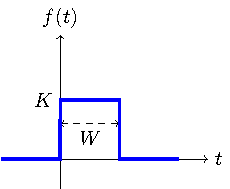
\includegraphics[width=.7\linewidth]{../figs/pulso.pdf}
        \end{center}
    \end{column}    
    \begin{column}{0.4\columnwidth}

        \vspace{6mm}
        
        $
            f(t) = %
            \begin{cases}
            0 & t < 0\\
            K & 0 \leq t \leq W\\
            0 & t>W
            \end{cases}
        $
    \end{column}
    \end{columns}
\end{frame}

%%%%%%%%%%%%%%%%%

\begin{frame}{Ecuaciones diferenciales} \label{diapo:RLC_serie_intro}
    \vspace{2mm}
    Al aplicar \alert{Kirchhoff} a un circuito lineal obtenemos ecuaciones diferenciales
    
    \[
      u_L(t) = L \; \diff{\,i_L(t)}{t}
      \quad\leftrightarrow\quad
      i_L(t) = \frac{1}{L} \int^t_{-\infty}u_L(\tau) \;d\tau
    \]
    
    \[
      i_C(t) = C \; \diff{\,u_C(t)}{t}
      \quad\leftrightarrow\quad
      u_C(t) = \frac{1}{C} \int^t_{-\infty}i_C(\tau) \;d\tau
    \]

    \vspace{3mm}
    Por ejemplo, la ecuación de un \alert{circuito RLC} serie será de la forma:
    
    \[
      L \; \diff[2]{i(t)}{t} + R \; \diff{\,i(t)}{t} + \frac{1}{C} \; i(t) = \diff{\,E(t)}{t}
    \]

    \vspace{1mm}
    \centering{\small(EDO lineal de segundo orden, obtenida aplicando 2LK al circuito)}
\end{frame}

%%%%%%%%%%%%%%%%%

\begin{frame}{Respuesta de un circuito lineal a una perturbación o consigna}

    \vspace{2mm}
    La \alert{solución} de la ecuación diferencial del circuito para \hspace{1.5mm}\(t \geq 0\) \hspace{2mm}(\textit{i.e.}, la \alert{respuesta del circuito} a la perturbación) \hspace{1mm}tiene \alert{dos componentes}\footnote{Esta es la solución general a una Ecuación Diferencial Ordinaria (EDO) lineal de orden arbitrario. Para más detalles, consultar \textit{e.g.} libro \href{https://ingenio.upm.es/primo-explore/fulldisplay?docid=34UPM_ALMA2169152810004212\&context=L&vid=34UPM_VU1\&lang=es_ES\&search_scope=TAB1_SCOPE1\&adaptor=Local\%20Search\%20Engine\&isFrbr=true\&tab=tab1\&query=any,contains,zill\%20ecuaciones\%20diferenciales\&offset=0}{Zill}}:
    
    \[
        \boxed{\;\; f(t) \;=\; f_n(t) \;+\; f_\infty(t) \;\;}
    \]

    \centering{\small(donde $f(t)$ puede referirse a tensión o corriente)}

    \normalsize
    \vspace{3mm}
    \begin{itemize}
        \item Respuesta \alert{natural} o propia, \hspace{3mm}\(f_n(t)\)

        \vspace{3mm}
        \item Respuesta \alert{forzada} o particular, \hspace{3mm}\(f_\infty(t)\)
    \end{itemize}
\end{frame}

%%%%%%%%%%%%%%%%%

\begin{frame}{Respuesta \textit{natural}, \hspace{3mm}$f_n(t)$}
    
    \begin{itemize}
        \item Respuesta \alert{natural} o propia, \hspace{3mm}\(f_n(t)\)

        \vspace{4mm}
        \begin{itemize}
        \normalsize
            \item Respuesta \alert{sin fuentes de alimentación} $\quad\rightarrow\quad$ solución de la \alert{ec. homogénea}

            \vspace{2mm}
            Volviendo al ejemplo del circuito RLC, la ec. homogénea sería:

            \vspace{-3mm}
            \[
              L \; \diff[2]{i(t)}{t} + R \; \diff{\,i(t)}{t} + \frac{1}{C} \; i(t) = \cancelto{0}{\diff{\,E(t)}{t}}
            \]

            \vspace{3mm}
            \item \(f_n(t)\) queda determinada por la \alert{energía almacenada previamente} (antes de conectar las fuentes) y por la \alert{topología del circuito} (conexiones entre elementos)

            \vspace{3mm}
            \item Contiene constantes de integración $\quad\rightarrow\quad$ necesario conocer el \alert{estado del circuito} en el instante que da origen al transitorio (\textit{i.e.}, las \underline{condiciones iniciales})
        \end{itemize}
    \end{itemize}
\end{frame}

%%%%%%%%%%%%%%%%%

\begin{frame}{Respuesta \textit{forzada}, \hspace{3mm}$f_\infty(t)$}

    \vspace{2mm}
    \begin{itemize}     
        \item Respuesta \alert{forzada} o particular, \hspace{3mm}\(f_\infty(t)\)

            \vspace{3mm}
            \begin{itemize}
                \normalsize

                \item Es una \alert{solución particular} a la ecuación diferencial \alert{no homogénea} $\quad\rightarrow\quad$
        
                \vspace{2mm}
                determinada por las fuentes existentes en \hspace{2mm}\(t > 0\), \hspace{3mm}${\boldsymbol{\color{blue!50!black} E(t)}}$ en el ejemplo RLC
                \begin{center}
                    \includegraphics[height=0.35\textheight]{../figs/RLC_serie_diapos.pdf}
                \end{center}   

                \vspace{3mm}
                \item Modela el estado del circuito \alert{tras un tiempo} suficientemente \alert{largo} después de 
                
                la perturbación (régimen permanente), ya que \underline{la respuesta natural se extingue} 
                \[
                    \hspace*{50mm} \lim_{t \to \infty} \;\, f_n(t) = 0
                    \qquad \textrm{\small(demostración más adelante)}
                \]
            \end{itemize}
    \end{itemize}
\end{frame}

%%%%%%%%%%%%%%%%%

\begin{frame}{Condiciones iniciales} \label{diapo:CondicionesIniciales}
    \begin{itemize}
        \item El \alert{instante del cambio} se representa habitualmente con \hspace{2mm}${\boldsymbol{\color{blue!50!black} t = 0}}$

        \begin{itemize}
            \normalsize
            \item \(t = 0^- \quad\rightarrow\quad \) tiempo inmediatamente \alert{anterior} al cambio

            \vspace{1mm}
            \item \(t = 0^+ \quad\rightarrow\quad \) tiempo inmediatamente \alert{posterior} al cambio
        \end{itemize}

        \vspace{5mm}
        \item Las \alert{condiciones iniciales} son el estado del circuito en \hspace{2mm}$t=0$

        \vspace{1mm}
        $\color{structure.fg}{\blacktriangleright}\;$ Se calculan con las \alert{energías almacenadas} en bobinas y condensadores en \hspace{2mm}$t=0^-$
        % Con "\color{structure.fg}" se usa el color del "theme" de Beamer

        \vspace{1mm}
        $\color{structure.fg}{\blacktriangleright}\;$ Se aplican a la \alert{topología} del circuito en \hspace{2mm}\(t = 0^+\)

        \vspace{6mm}
        \item Las cond. iniciales determinan las \alert{ctes. de integración} de la respuesta \alert{natural}, \hspace{1mm}\(f_n(t)\)
    \end{itemize}
\end{frame}

%%%%%%%%%%%%%%%%%

\begin{frame}{Condiciones iniciales, \hspace{3mm}resistencia}
    \alert{No acumula energía} $\quad\rightarrow\quad$ sigue los cambios de forma instantánea

    \vspace{1mm}
    \[
        u(t) = R\cdot i(t)
    \]

    \vspace{2mm}
    \centering{(no aparece ninguna derivada en su ec. de definición)}
\end{frame}

%%%%%%%%%%%%%%%%%

\begin{frame}{Condiciones iniciales, \hspace{3mm}bobina} \label{diapo:continuidad_L}

    Para aplicar la \alert{condición inicial} de la bobina (\textit{i.e.}, \alert{energía almacenada} en $t=0^-$) a la topología del circuito en  $t=0^+$, basta con considerar la \alert{\textit{condición de continuidad}}: 

    \begin{center}
        \underline{No son posibles} tensiones infinitas ni corrientes infinitas
    \end{center}
    
        Según la ec. de definición de la bobina, la \alert{corriente no puede variar de forma brusca} (implicaría tensión infinita):
        \[
            u_L(t) = L \; \diff{\, i_L(t)}{t}
            \quad\Rightarrow\quad        
            \boxed{\; i_L(0^-) = i_L(0^+) \;}
        \]
    
    Si la corriente cambiara de forma brusca, su derivada sería infinita (por ejemplo, \hyperlink{diapo:escalon}{función escalón}) $\;\,\rightarrow\;\,$ la tensión en bornes sería infinita (\alert{físicamente imposible})
    
\end{frame}

%%%%%%%%%%%%%%%%%

\begin{frame}{Condiciones iniciales, \hspace{3mm}condensador} \label{diapo:continuidad_C}
    Para aplicar la \alert{condición inicial} del condensador (\textit{i.e.}, \alert{energía almacenada} en $t=0^-$) a la topología del circuito en  $t=0^+$, basta con considerar la \alert{\textit{condición de continuidad}}: 

    \begin{center}
        \underline{No son posibles} tensiones infinitas ni corrientes infinitas
    \end{center}
    
        Según la ec. de definición del condensador, la \alert{tensión no puede variar de forma brusca} (implicaría corriente infinita):
        \[
            i_C(t) = C \; \diff{\, u_C(t)}{t}
            \quad\Rightarrow\quad        
            \boxed{\; u_C(0^-) = u_C(0^+) \;}
        \]
    
    Si la tensión cambiara de forma brusca, su derivada sería infinita (por ejemplo, \hyperlink{diapo:escalon}{función escalón}) $\;\,\rightarrow\;\,$ la corriente de carga o
    descarga sería infinita (\alert{físicamente imposible})
\end{frame}

%%%%%%%%%%%%%%%%%

%\begin{frame}{Condiciones iniciales}{Ejemplo}
%    En la red de la figura, la corriente del generador de intensidad es $i_g(t) = 10\,\mathrm{e}^{-2t}$ A. El interruptor se abre en $t = 0$, siendo los valores iniciales $i_L(0^-) = 0$ A; $u_C(0^-) = -5$ V. Se pide calcular $i_R(0^+)$, $i_C(0^+)$ y $u_L(0^+)$
%\begin{figure}[H]
%    \centering
%    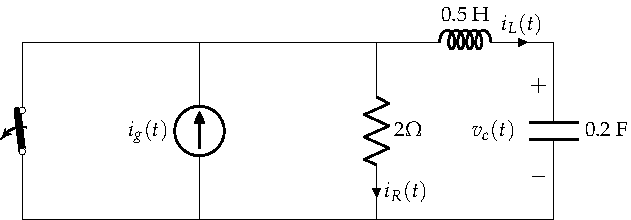
\includegraphics{../figs/ej_condiciones_iniciales.pdf}
%\end{figure}
%\end{frame}

%%%%%%%%%%%%%%%%%

\section{Circuitos de primer orden}

\begin{frame}{Circuitos de primer orden: \hspace{3mm}definición}
    \vspace{3mm}
    \begin{itemize}
        \item Circuitos compuestos por:
        \vspace{2mm}
        \begin{itemize}
            \normalsize
            \item Un \alert{único elemento de acumulación} (o varios elementos que pueden ser simplificados a un elemento equivalente, \textit{e.g.} bobinas en serie) 

            \vspace{2mm}
            \item Y \alert{resistencias}
        \end{itemize}
        
        \vspace{5mm}
        \item Modelados mediante una \alert{ec. diferencial de} ${\boldsymbol{\color{blue!50!black} 1^{\textrm{er}}}}$ \alert{orden}:   

        \vspace{1mm}
        \begin{equation*}
           \boxed{\; a_1\cdot f'(t) \,+\, a_0\cdot f(t) \,=\, g(t) \;}
        \end{equation*}
        
        \begin{equation*}
            \textrm{ejemplo de RL serie:} \qquad L\cdot i'(t) \,+\, R\cdot i(t) \,=\, E(t)
        \end{equation*}
    \end{itemize}
\end{frame}

%%%%%%%%%%%%%%%%%

\begin{frame}{Circuitos de primer orden: \hspace{3mm}resolución} \label{diapo:pasos_PrimerOrden}
    \vspace{2mm}
    \begin{itemize}
        \item Modelados mediante una \alert{ec. diferencial de} ${\boldsymbol{\color{blue!50!black} 1^{\textrm{er}}}}$ \alert{orden}:   

        \vspace{1mm}
        \begin{equation*}
           \boxed{\; a_1\cdot f'(t) \,+\, a_0\cdot f(t) \,=\, g(t) \;}
        \end{equation*}
        
        \begin{equation*}
            \textrm{ejemplo de RL serie:} \qquad L\cdot i'(t) \,+\, R\cdot i(t) \,=\, E(t)
        \end{equation*}

        \vspace{1mm}
        \item $\boxed{\; \textrm{Resolución} \;}$

        \vspace{2mm}
        \begin{enumerate}
            \normalsize
            \item Cálculo de las \alert{condiciones iniciales}, analizando el circuito en \(\,t=0^-\)

            \vspace{2mm}
            \item \alert{Respuesta natural}: análisis de la \alert{ec. homogénea} ($g(t)=0$, \underline{sin fuentes}) en \(\, t>0\)
            \begin{equation*}
                \hspace*{50mm} f_n(t) = K\cdot\mathrm{e}^{-\dfrac{a_0}{a_1}\, \scalebox{2} {\tiny \textit{t}}} \qquad \textrm{\small(demostración a continuación)}
            \end{equation*}

            \normalsize
            \vspace{2mm}
            \item \alert{Respuesta forzada}, $f_\infty(t)$: análisis del circuito \underline{con fuentes} en \(\, t>0\)
        \end{enumerate}
    \end{itemize}
\end{frame}

%%%%%%%%%%%%%%%%%

\subsection{Circuito RL serie}

\begin{frame}{Circuito RL serie básico}
    \vspace{3mm}
    \begin{itemize}
        \item En \(\; t < 0 \;\) la fuente está desconectada
        \item En \(\; t = 0 \;\) la fuente se conecta
        \item En \(\; t > 0 \;\) la fuente alimenta el circuito RL (la bobina almacena energía)
    \end{itemize}

    \begin{center}
        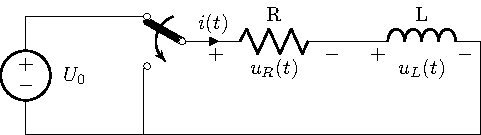
\includegraphics[height=0.6\textheight]{../figs/transitorio_circuitoRL.pdf}
    \end{center}
\end{frame}

%%%%%%%%%%%%%%%%%

\begin{frame}{Condiciones iniciales} \label{diapo:CondicionInicialRL}
    Analizando el circuito para \(\; t < 0\) \ldots{}
    \begin{center}
        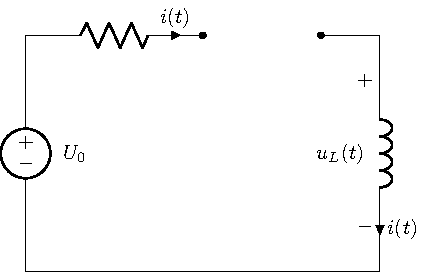
\includegraphics[height=0.57\textheight]{../figs/transitorio_circuitoRL_t0-.pdf}
    \end{center}
    \ldots{}obtenemos \( \;\boxed{\; i(0^-) = 0 \;}\)  
\end{frame}

%%%%%%%%%%%%%%%%%

\begin{frame}{Respuesta natural, \hspace{3mm}$f_n(t)$}
    Siguiendo los pasos de la diapositiva~\ref{diapo:pasos_PrimerOrden}, analizamos el circuito para $t>0$ \alert{apagando la fuente} (ec. homogénea):
    \begin{columns}
    \begin{column}{0.5\columnwidth}
        \begin{center}
            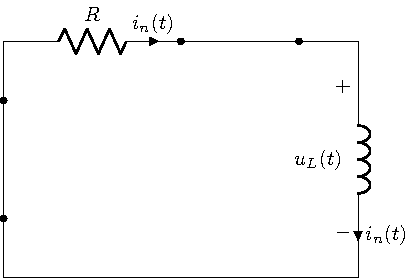
\includegraphics[height=0.55\textheight]{../figs/transitorio_circuitoRL_t0+_Natural.pdf}
        \end{center}
    \end{column}
    \begin{column}{0.5\columnwidth}
        \vspace{5mm}
        \[
          \hspace*{-20mm} \textrm{\alert{2LK}} \quad\rightarrow\quad u_R(t) \,+\, u_L(t) \, = \, 0
        \]
        
        \vspace{2mm}
        Sustituyendo las \alert{ecs. de definición} de $R$ y $L$:
        
        \[
          \hspace*{5mm} R \cdot i_n(t) \,+\, L \; \diff{\,i_n(t)}{t} \, = \,  0
        \]

        \vspace{2mm}
        Cuya \alert{solución general} es:
        \[
          \boxed{\; i_n(t) \,=\, K \cdot e^{\,s\,t} \;}
        \]
        \centering{\small(deducción en la siguiente diapositiva)}
    \end{column}
    \end{columns}    
\end{frame}

%%%%%%%%%%%%%%%%%

\begin{frame}{Respuesta natural, \hspace{3mm}$f_n(t)$} \label{diapo:deduccion_PrimerOrden}
    \vspace{3mm}
    La ec. homogénea a resolver es:  

    \vspace{-5mm}
    \[
      L \; \diff{\,i_n(t)}{t} \,+\, R \cdot i_n(t) \, = \,  0
    \]
    
    Para resolverla, debe hallarse una función cuya \alert{derivada sea igual a la propia función}, multiplicada por una constante $\;\;\rightarrow\;\;$ la \alert{función exponencial} cumple esta propiedad 

    \vspace{4mm}
    \alert{Sustituyendo} entonces $\; i_n(t) = K \cdot e^{\,s\,t} \;$ (donde ${\boldsymbol{\color{blue!50!black} K}}$ y ${\boldsymbol{\color{blue!50!black} s}}$ son \alert{constantes} a determinar):
    \[
      L \; \diff{\,(K \cdot e^{\,s\,t})}{t} \,+\, R \cdot K \cdot e^{\,s\,t} \, = \,  0 
      \quad\rightarrow\quad 
      s \cdot K \cdot e^{\,s\,t} \,+\, \frac{R}{L} \cdot K \cdot e^{\,s\,t}   \, = \,  0
    \]
    Diviendo a ambos lados por $\; K \cdot e^{\,s\,t} \;$ se obtiene la  \alert{ec. característica}:
    \[
      s + \frac{R}{L} = 0 
      \quad\rightarrow\quad
      s = -\frac{R}{L}       
      \quad \xrightarrow[i_n(t) \,=\, K \cdot \, e^{\,s\,t}]{\quad \textrm{sustituyendo en} \quad} \quad
      \boxed{\; \vphantom{\dfrac{a}{a}} i_n(t) \,=\, K \cdot e^{\,-\frac{\vphantom{j} \scalebox{1.5} {\tiny \textit{R}}}{\vphantom{\scalebox{2} {\tiny \textit{L}}} \scalebox{1.5} {\tiny \textit{L}}} \,\scalebox{1.5} {\tiny \textit{t}}} \;}
    \]

    \blfootnote{Para más detalles, consultar págs. 400 - 404 del \href{https://ingenio.upm.es/primo-explore/fulldisplay?docid=34UPM_ALMA2150534070004212\&context=L\&vid=34UPM_VU1\&lang=es_ES\&search_scope=TAB1_SCOPE1\&adaptor=Local\%20Search\%20Engine\&isFrbr=true\&tab=tab1\&query=any,contains,circuitos\%20electricos\%20fraile\%20mora\&sortby=date\&facet=frbrgroupid,include,578542795\&offset=0}{Fraile Mora}, edición 2012}
\end{frame}

%%%%%%%%%%%%%%%%%

\begin{frame}{Respuesta natural, \hspace{3mm}$f_n(t) \quad\rightarrow\quad$ constante de tiempo}
    \begin{columns}
    \begin{column}{0.42\linewidth}
        Definimos \(\, \tau = \dfrac{L}{R} \;\) como la \alert{constante} 

        \vspace{2mm}
        \alert{de tiempo} del circuito (unidades [s])    
        \[
          \boxed{\; i_n(t) \,=\, K \cdot e^{-t/\tau} \;}
        \]
        
        \begin{itemize}
            \item Ratio entre \alert{almacenamiento} (\(L\)) y \alert{disipación} (\(R\))
    
            \vspace{3mm}
            \item Valores altos de \(\tau\) implican decrecimiento lento
    
            \vspace{3mm}
            \item La respuesta natural \alert{se extingue} tras \(\; \simeq 5\tau\)
        \end{itemize}
    \end{column}
    \begin{column}{0.58\linewidth}
        \vspace{2mm}
        \begin{center}
            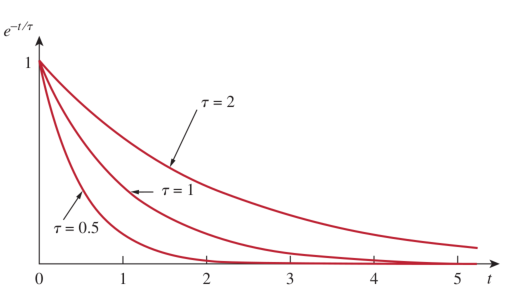
\includegraphics[height=0.6\textheight]{../figs/constante_tiempo.pdf}
        \end{center}

        \hspace{5mm}La \alert{energía almacenada} en la bobina en $t=0^-$ 
        
        \hspace{5mm}se \alert{disipa en las resistencias} en $t>0$
    \end{column}
    \end{columns}
\end{frame}

%%%%%%%%%%%%%%%%%

\begin{frame}{Respuesta forzada, \hspace{3mm}$f_\infty(t)$}
    
    \vspace{3mm}
    Volvemos a \alert{activar la fuente}, analizando para $t>0$:
    \begin{columns}
    \begin{column}{0.5\columnwidth}

        \vspace{-5mm}
        \begin{center}
            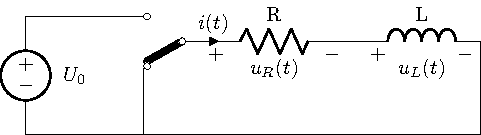
\includegraphics[height=0.55\textheight]{../figs/transitorio_circuitoRL_t0+.pdf}
        \end{center}
    \end{column}
    \hfill
    \begin{column}{0.48\columnwidth}
        \vspace{-1mm}
        \begin{align*}
          \hspace*{-16mm} \textrm{\alert{2LK}} \quad\rightarrow\quad 
          u_R(t) \,&+\, u_L(t) \, = \, u(t) \\[5pt] 
          R \; i(t) \,&+\, L\; \cancelto{0\, \textrm{(CC)}}{\diff{\, i(t)}{t}} \, = \, U_0
        \end{align*}

        \vspace{4mm}    
        Al ser un circuito de \alert{Corriente Continua}, la \alert{bobina} se sustituye por un \alert{cortocircuito}

        \vspace{6mm} 
        La \alert{solución} es entonces:
        \begin{equation*}
            \boxed{\; i_\infty(t) \,=\, \frac{U_0}{R} \;}
        \end{equation*}
        
    \end{column}
    \end{columns}  
\end{frame}

%%%%%%%%%%%%%%%%%

\begin{frame}{Respuesta completa, \hspace{3mm}$f(t) \;=\; f_n(t) \;+\; f_\infty(t)$}
    \begin{equation*}
        i(t) \,=\, i_n(t) \,+\, i_\infty(t) \;\,\rightarrow\;\,
        \begin{cases}
            \, i_n(t) \,=\, K \cdot e^{-t/\tau}\\[3pt]
            \, i_\infty(t) \,=\, U_0/R\\
        \end{cases}
    \end{equation*}
    
    Para \alert{determinar} el valor de la \alert{constante de integración} $\, K \,$, \hyperlink{diapo:CondicionesIniciales}{particularizamos en \(t = 0^+\)}:
    \begin{equation*}
        i(0^+) \,=\, i_n(0^+) \,+\, i_\infty(0^+) \,=\, K \,+\, \frac{U_0}{R} \quad\rightarrow\quad K \,=\, i(0^+) \,-\, i_\infty(0^+)
    \end{equation*}
    Teniendo en cuenta la \alert{condición de continuidad}, \(\; i(0^+) \,=\,\) \hyperlink{diapo:CondicionInicialRL}{\(\, i(0^-) \,=\, 0 \)} , obtenemos:
    \[
        K \,=\, 0 \,-\, \frac{U_0}{R}
    \]
    La \alert{solución completa} (para \underline{esta topología concreta}) es :
    \[
        \boxed{ \vphantom{\frac{\frac{a}{a}}{\frac{a}{a}}}\;\; i(t) \,=\, \frac{U_0}{R} \,\left(1 \,-\, e^{-t/\tau} \right) \;\;}
    \]
\end{frame}

%%%%%%%%%%%%%%%%%

\begin{frame}{Respuesta completa, \hspace{3mm}$f(t) \;=\; f_n(t) \;+\; f_\infty(t)\,$, \hspace{3mm}para esta topología} \label{diapo:RL_resultado}
    \Large
    \[
        \boxed{ \vphantom{\frac{\frac{a}{a}}{\frac{a}{a}}}\;\; i(t) \,=\, \frac{U_0}{R} \,\left(1 \,-\, e^{-t/\tau} \right) \;\;}
    \]
    
    \begin{center}
        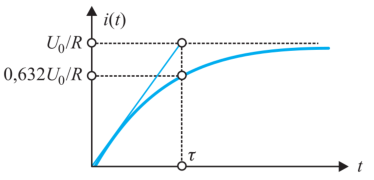
\includegraphics[height=0.45\textheight]{../figs/RespuestaCompleta_RL.pdf}
    \end{center}
\end{frame}

%%%%%%%%%%%%%%%%%

\begin{frame}{Expresión \underline{general} de la respuesta completa}

    La \alert{respuesta completa} de un \alert{circuito RL general} (\textit{i.e.}, para \underline{cualquier topología})
    
    \large
    \[
        \boxed{\;\; i(t) \;\;=\;\; \overbrace{\underbrace{\left[i(0^+) \,-\, i_\infty(0^+)\right]}_{\vphantom{\frac{a}{a}} =K} \cdot \, e^{-t/\tau}}^{\vphantom{\frac{A}{A}} i_n(t)} \;\;+\;\; i_\infty(t) \;\;}
    \]

    \vspace{2mm}
    \normalsize
    \begin{itemize}
        \item \(i(0^+) \;\;\rightarrow\;\) corriente en la bobina en \(t = 0^+\), definida por cond. iniciales, \(i(0^-) = i(0^+)\)

        \vspace{2mm}
        \item \(i_\infty(t) \hspace{2.5mm}\rightarrow\;\) corriente en la bobina en régimen permanente (para \(\, t > 0 \))

        \vspace{2mm}
        \item \(i_\infty(0^+) \hspace{-0.25mm}\rightarrow\;\) corriente en la bobina, en régimen permanente, en \(\, t = 0^+\)
    \end{itemize}
\end{frame}

%%%%%%%%%%%%%%%%%

\subsection{Circuito RC paralelo}

\begin{frame}{Circuito RC paralelo básico}
    \vspace{1mm}
    \begin{itemize}
        \item En \(\; t < 0 \;\) la fuente alimenta el circuito RC (el condensador se carga)
        \item En \(\; t = 0 \;\) se desconecta la fuente
        \item En \(\; t > 0 \;\) el condensador comienza a descargarse en la resistencia
    \end{itemize}
    
    \begin{center}
        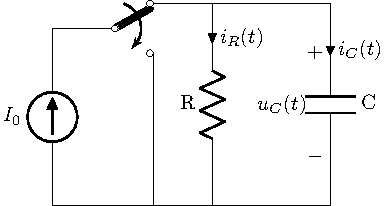
\includegraphics[height=0.47\textheight]{../figs/transitorio_circuitoRC.pdf}
    \end{center}
\end{frame}

%%%%%%%%%%%%%%%%%

\begin{frame}{Condiciones iniciales} \label{diapo:CondicionInicialRC}
    Analizando el circuito para \(\; t < 0\) \ldots{}
    \begin{center}
        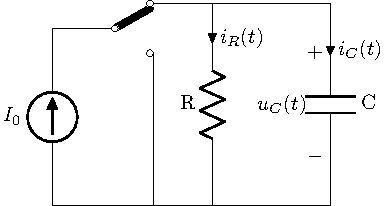
\includegraphics[height=0.47\textheight]{../figs/transitorio_circuitoRC_t0-.pdf}
    \end{center}
    \ldots{}obtenemos \( \;\boxed{\; u_C(0^-) \,=\, R \cdot I_0 \;}\)
\end{frame}

%%%%%%%%%%%%%%%%%

\begin{frame}{Respuesta natural, \hspace{3mm}$f_n(t)$}
     \vspace{3mm}
    Siguiendo los pasos de la diapositiva~\ref{diapo:pasos_PrimerOrden}, analizamos el circuito para $t>0$ \alert{apagando la fuente} (ec. homogénea)

    \vspace{-10mm}
    
    \begin{columns}
    \begin{column}{0.45\columnwidth}

        \vspace{9mm}
        \begin{center}
            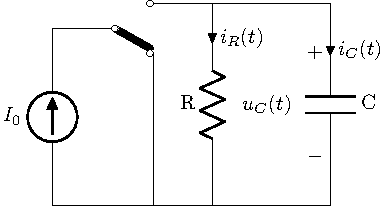
\includegraphics[height=0.42\textheight]{../figs/transitorio_circuitoRC_t0+.pdf}
        \end{center}
        
        \begin{center}
            {\small(en este caso, la fuente 
            
            ya está apagada en $t>0$)}
        \end{center}
    \end{column}
    \begin{column}{0.55\columnwidth}
        \vspace{5mm}
        \begin{align*}
          \hspace*{-20mm} \textrm{\alert{1LK}} \quad\rightarrow\quad i_R(t) \,&+\, i_C(t) \,=\, 0 \\[3pt]
          \hspace*{5mm} \frac{u_n(t)}{R} \,&+\, C \;\diff{\, u_n(t)}{t} \,=\, 0
        \end{align*}

        \vspace{1mm}
        Cuya \alert{solución general} es:

        \vspace{-2mm}
        \[
          \boxed{\; u_n(t) \,=\, K \cdot e^{\,s\,t} \;}
        \]
        \begin{center}
            {\small(deducción equivalente a la diapositiva \ref{diapo:deduccion_PrimerOrden})}
        \end{center}

        \vspace{1mm}
        Luego la \alert{respuesta natural}, $\, u_n(t)\,$ del circuito es: 

        \vspace{-2mm}
        \[
          \boxed{\; \vphantom{\dfrac{a}{a}} u_n(t) \,=\, K \cdot e^{\,-\frac{\vphantom{j} \scalebox{1.5} {\tiny \textit{t}}}{\vphantom{\scalebox{2} {\tiny \textit{R C}}} \scalebox{1.5} {\tiny \textit{R$\cdot$C}}}} \;}
        \]
    \end{column}
    \end{columns}  
\end{frame}

%%%%%%%%%%%%%%%%%

\begin{frame}{Respuesta natural, \hspace{3mm}$f_n(t) \quad\rightarrow\quad$ constante de tiempo}
    \begin{columns}
    \begin{column}{0.45\linewidth}

        \vspace{-14mm}
        Definimos \(\, \tau = R\cdot C \;\) como la \alert{constante} 

        \vspace{1mm}
        \alert{de tiempo} del circuito (unidades [s])    
        \[
          \boxed{\; u_n(t) \,=\, K \cdot e^{-t/\tau} \;}
        \]
        
        \begin{itemize}
            \item Valores altos de \(\tau\) implican decrecimiento lento
    
            \vspace{3mm}
            \item La respuesta natural \alert{se extingue} tras \(\; \simeq 5\tau\)
        \end{itemize}
    \end{column}
    \begin{column}{0.55\linewidth}
        \vspace{-1mm}
        \begin{center}
            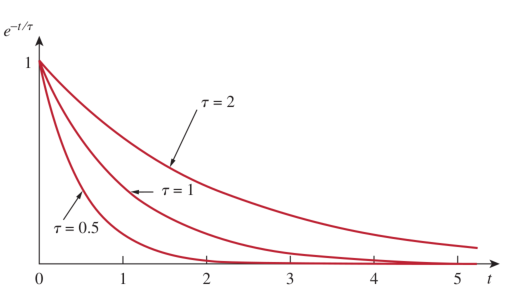
\includegraphics[height=0.57\textheight]{../figs/constante_tiempo.pdf}
        \end{center}

        \hspace{5mm}La \alert{energía almacenada} en el $C$ en $t=0^-$ 
        
        \hspace{5mm}se \alert{disipa en las resistencias} en $t>0$
    \end{column}
    \end{columns}
\end{frame}

%%%%%%%%%%%%%%%%%

\begin{frame}{Respuesta forzada, \hspace{3mm}$f_\infty(t)$}
    
    \vspace{-3mm}
    Analizando para $t>0$ con la \alert{fuente encendida}:

    \vspace{3mm}
    \begin{columns}
    \begin{column}{0.4\columnwidth}

        \vspace{5mm}
        
        \hspace*{-3mm}
        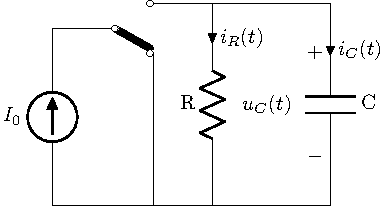
\includegraphics[height=0.42\textheight]{../figs/transitorio_circuitoRC_t0+.pdf}
    \end{column}
    \hfill
    \begin{column}{0.52\columnwidth}
        \vspace{5mm}

        Dado que en $t>0$ \alert{no hay fuentes} presentes en el circuito RC, toda la \alert{energía almacenada} en el condensador \alert{se disipa} en la resistencia

        \vspace{9mm}
        Luego la \alert{respuesta forzada}, $\; u_\infty(t) \,$, es:
        
        \begin{equation*}
            \boxed{\; u_\infty(t) \,=\, 0 \;}
        \end{equation*}
        
    \end{column}
    \end{columns}  
\end{frame}

%%%%%%%%%%%%%%%%%

\begin{frame}{Respuesta completa, \hspace{3mm}$f(t) \;=\; f_n(t) \;+\; f_\infty(t)$} \label{diapo:RC_resultado}
    \begin{equation*}
        u(t) \,=\, u_n(t) \,+\, u_\infty(t) \;\,\rightarrow\;\,
        \begin{cases}
            \, u_n(t) \,=\, K \cdot e^{-t/\tau}\\[3pt]
            \, u_\infty(t) \,=\, 0\\
        \end{cases}
    \end{equation*}
    
    Para \alert{determinar} el valor de la \alert{constante de integración} $\, K \,$, \hyperlink{diapo:CondicionesIniciales}{particularizamos en \(t = 0^+\)}:
    \begin{equation*}
        u(0^+) \,=\, u_n(0^+) \,+\, u_\infty(0^+) \,=\, K \,+\, 0 \quad\rightarrow\quad K \,=\, u(0^+)
    \end{equation*}
    Teniendo en cuenta la \alert{condición de continuidad}, \(\; u(0^+) \,=\,\) \hyperlink{diapo:CondicionInicialRC}{\(\, u(0^-) \,=\, R \cdot I_0 \)} \(\,=\, U_0 \, \):
    \[
        K \,=\, U_0
    \]
    La \alert{solución completa} (para \underline{esta topología concreta}) es :
    \[
        \boxed{ \vphantom{\frac{\frac{a}{a}}{\frac{a}{a}}}\;\; u(t) \,=\, U_0 \cdot e^{-t/\tau} \;\;}
    \]
\end{frame}

%%%%%%%%%%%%%%%%%

\begin{frame}{Balance energético}
    Podemos comprobar que \alert{toda la energía} acumulada en el condensador en \(\, t < 0 \,\) 

    realmente \alert{se disipa} en la resistencia en \(\, t > 0 \,\):
    
    \begin{align*}
      \boxed{\; W_R \;} \;&=\; 
      \int_0^\infty u_R(t)\cdot i_R(t) \;\mathrm{d}t 
      \;=\; \int_0^\infty \frac{u_R^2(t)}{R} \;\mathrm{d}t 
      \;=\; \int_0^\infty \frac{1}{R} \, (U_0 \cdot e^{-t/\tau})^2  \;\mathrm{d}t 
      \;=\; \\[8pt]
      &=\;  \frac{U_0^2}{R} \int_0^\infty e^{\,- \frac{\vphantom{j} \scalebox{1.5} {\tiny 2}}{\vphantom{\scalebox{2} {\tiny \textit{R C}}} \scalebox{1.5} {\tiny \textit{R$\cdot$C}}}\,\scalebox{1.5} {\tiny \textit{t}} }  \;\mathrm{d}t 
      \;=\;
      \frac{U_0^2}{\cancel{R}} \cdot \frac{-\cancel{R}\cdot C}{2} \, \left[ e^{\,- \frac{\vphantom{j} \scalebox{1.5} {\tiny 2}}{\vphantom{\scalebox{2} {\tiny \textit{R C}}} \scalebox{1.5} {\tiny \textit{R$\cdot$C}}}\,\scalebox{1.5} {\tiny \textit{t}} } \right]^{\infty}_0
      \;=\; 
      \frac{-1}{2} \; C \cdot U_0^2 \cdot [0 \,-\, 1]
      \\[8pt]
      &=\; \frac{1}{2} \; C \cdot U_0^2 \;=\; \boxed{\; W_C \;}  
    \end{align*}
\end{frame}

%%%%%%%%%%%%%%%%%

\begin{frame}{Expresión \underline{general} de la respuesta completa}

    La \alert{respuesta completa} de un \alert{circuito RC general} (\textit{i.e.}, para \underline{cualquier topología})
    
    \large
    \[
        \boxed{\;\; u(t) \;\;=\;\; \overbrace{\underbrace{\left[u(0^+) \,-\, u_\infty(0^+)\right]}_{\vphantom{\frac{a}{a}} =K} \cdot \, e^{-t/\tau}}^{\vphantom{\frac{A}{A}} u_n(t)} \;\;+\;\; u_\infty(t) \;\;}
    \]

    \vspace{2mm}
    \normalsize
    \begin{itemize}
        \item \(u(0^+) \;\;\rightarrow\;\) tensión en el $C$ en \(\, t = 0^+\), definida por las cond. iniciales, \(\, u(0^-) = u(0^+)\)

        \vspace{2mm}
        \item \(u_\infty(t) \hspace{2.5mm}\rightarrow\;\) tensión en el $C$ en régimen permanente (para \(\, t > 0 \))

        \vspace{2mm}
        \item \(u_\infty(0^+) \hspace{-0.25mm}\rightarrow\;\) tensión en el $C$, en régimen permanente, en \(\, t = 0^+\)
    \end{itemize}
\end{frame}

%%%%%%%%%%%%%%%%%

\subsection{Procedimiento general}

\begin{frame}{Procedimiento general $\quad\rightarrow\quad$ equivalente de Thévenin/Norton}
    \vspace{0.5mm}

    \hspace{13mm}
    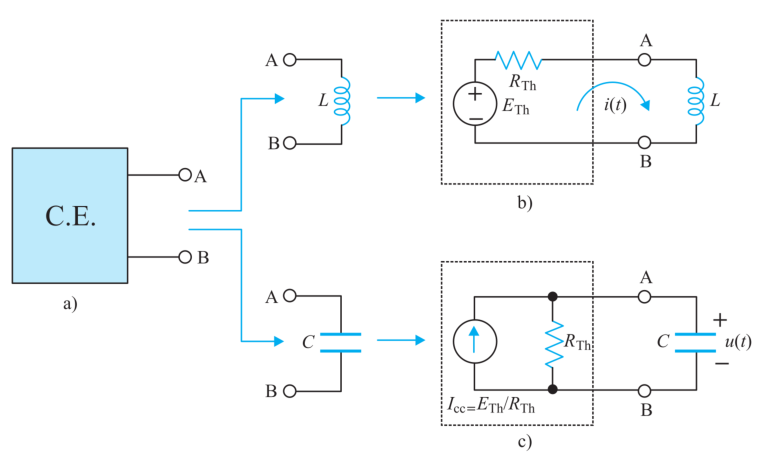
\includegraphics[height=0.82\textheight]{../figs/Thevenin_PrimerOrden.pdf}

    \vspace{-3mm}
    $R_{th}$ es la \alert{resistencia vista desde los bornes} del condensador o de la bobina, cuando se anulan todas las fuentes independientes
\end{frame}

%%%%%%%%%%%%%%%%%

\begin{frame}{Procedimiento general}
    \vspace{3mm}
    \begin{enumerate}
        \item Dibujar el circuito para ${\boldsymbol{\color{blue!50!black} \, t < 0 \,}}$
        \begin{itemize}
            \normalsize

            \vspace{2mm}
            \item Obtener el valor de \(\, i_L(0^-) \,\) o \(\, u_C(0^-) \,\)

            \vspace{2mm}
            \item Aplicar el \alert{principio de continuidad} para determinar \(\, i_L(0^+) \,\) o \(\, u_C(0^+) \,\)
        \end{itemize}

        \vspace{4mm}
        \item Dibujar el circuito para ${\boldsymbol{\color{blue!50!black} \, t > 0 \,}}$
        \begin{itemize}
            \normalsize

            \vspace{1mm}
            \item Calcular el equivalente de \alert{Thévenin/Norton} visto por $L$ o $C$

            \vspace{2mm}
            \item Determinar la \alert{constante de tiempo} del circuito:
            $\quad \tau = \dfrac{L}{R_{th}} \quad\textrm{o}\quad \tau = R_{th}\cdot{C}$

            \vspace{2mm}
            \item Calcular la respuesta en \alert{régimen permanente}, \(\, i_\infty(t) \,\) o \(\, u_\infty(t) \,\)
        \end{itemize}

        \vspace{3mm}
        \item Obtener la \alert{respuesta completa}:
    \end{enumerate}

    \vspace{-6mm}
    \begin{align*}
        i_L(t) \;\;&=\;\; \left[i_L(0^+) \,-\, i_\infty(0^+)\right] \cdot \, e^{-t/\tau} \;\;+\;\; i_\infty(t)\\[4pt]
        u_C(t) \;\;&=\;\; \left[u_C(0^+) \,-\, u_\infty(0^+)\right] \cdot \, e^{-t/\tau} \;\;+\;\; u_\infty(t)\\
    \end{align*}
\end{frame}

%%%%%%%%%%%%%%%%%

%\begin{frame}{Circuitos de primer orden}{Ejemplo 1}
%    \textbf{En el circuito de la figura, calcular la corriente $i(t)$ al cerrar el interruptor en $t = 0$ s.}
%	    \begin{figure}[H]
%	        \centering
%	        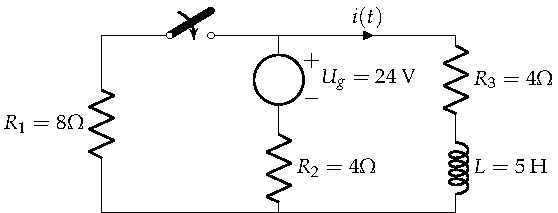
\includegraphics{../figs/ej_transitorio_1orden.pdf}
%	    \end{figure}
%\end{frame}

%%%%%%%%%%%%%%%%%

%\begin{frame}{Circuitos de primer orden}{Ejemplo 2}
%    \textbf{El conmutador del circuito de la figura pasa de la posición a 1 a la 2 en $t = 0$ s. Calcular la tensión en bornes de la bobina $t > 0$ s.}
%	
%	\begin{figure}[H]
%	    \centering
%	    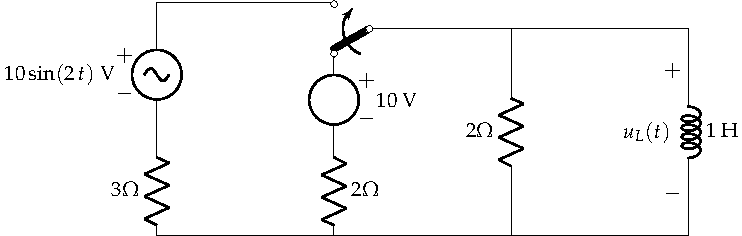
\includegraphics{../figs/ej_transitorio_1orden_AC.pdf}
%	\end{figure}
%\end{frame}

%%%%%%%%%%%%%%%%%

\begin{frame}{\underline{Resumen}: \hspace{3mm}respuestas posibles de un $1^{\textrm{er}}$ orden \hspace{3mm}(corriente continua)}

\vspace{3mm}
    \begin{minipage}[c]{0.47\linewidth} 

        Elemento que se \alert{descarga} (parcialmente)        
        % El elemento de acumulación tenía energía, la pierde parcialmente, y se queda en otro nivel de energía (nota: el caso en el que la pierde totalmente, porque no hay respuesta forzada, es caso particular de este)

        \vspace{3mm}
        \includegraphics[width=1\linewidth]{../figs/soluciones_1erOrden_Caso1.pdf}

        \vspace{3mm}
        \alert{Caso particular}: \hyperlink{diapo:RC_resultado}{$A=0$}, no hay fuentes en $t>0 \,$ (el elemento se \alert{descarga totalmente})
    \end{minipage}
    \hfill
    \vrule
    \hfill
    \begin{minipage}{0.47\linewidth} 
        Elemento ($C$ o $L$) que \alert{aumenta su carga} 
        % El elemento de acumulación tenía energía, pero tras la perturbación, está sometido a mayor tensión (para C) o circula más corriente (para L) que en el momento previo a la perturbación, así que aumenta la energía que almacena (nota: el caso en el que el elemento de acumulación no tuviera nada de energía almacenada es caso particular de este).
        
        \vspace{3mm}
        \includegraphics[width=1\linewidth]{../figs/soluciones_1erOrden_Caso2.pdf}
        
        \vspace{3mm}
        \alert{Caso particular}: \hyperlink{diapo:RL_resultado}{$C=D$}, el elemento % de acumulación 
        estaba \alert{inicialmente descargado}
    \end{minipage}

    % La respuesta natural es debida al cambio en la topología del circuito (nuevas conexiones), pero sin fuentes, que por tanto se centra en cómo se redistribuye la energía previamente almacenada en condensadores y bobinas. Por eso hay que considerar el circuito en t=0+

    % Si no hubiera energía previamente almacenada, lo que nos dice la respuesta natural es cómo se va a acumular la energía en el elemento de acumulación (por ejemplo, el circuito RL serie que hay en las diapos)
\end{frame}

%%%%%%%%%%%%%%%%%

\begin{frame}[plain]{Interludio: \hspace{17mm}transitorios inestables, \hspace{10mm}\href{https://en.wikipedia.org/wiki/Northeast_blackout_of_2003}{apagón EE. UU. 2003}}
    \begin{minipage}[c]{0.49\linewidth} 
        
        \vspace{3mm}
        
        \begin{itemize}
            \item \alert{55 millones} de personas sin luz 

            \vspace{1mm}
            \item \alert{6.000 millones de \$} en pérdidas
            % Reference: https://ieeexplore.ieee.org/document/10105838
        \end{itemize}

        \vspace{0mm}
           
        \hspace{-5mm}    
        \includegraphics[width=0.90\linewidth]{../figs/Map_of_North_America_blackout_2003.pdf}
        
    \end{minipage}
    \hfill%
    \begin{minipage}[c]{0.5\linewidth}    
    
        \vspace{-10mm}
        \begin{adjustwidth}{-0.5cm}{}% Necesita "\usepackage{changepage}"
        \begin{itemize}
            \item \alert{Nueva York} perdió gran parte del suministro durante \alert{13 horas} 
    
            \vspace{2mm}
            \item Ocurrió en agosto a las 16h: \alert{podría haber sido mucho peor} (\textit{e.g.}~diciembre a las 16h, sin luz natural)
        \end{itemize}
        \end{adjustwidth}

        \vspace{2mm}

        \hspace{-1mm} 
        \includegraphics[width=1\linewidth]{../figs/NYC_blackout.jpg}        
    \end{minipage}
\end{frame}

%%%%%%%%%%%%%%%%%

\section{Circuitos de segundo orden}

\begin{frame}{Circuitos de segundo orden}
    \begin{itemize}
        \item Circuitos que contienen \alert{dos elementos de acumulación}, además de elementos de disipación (resistencias) 

        \vspace{5mm}
        \item Modelados mediante una \alert{ec. diferencial de} ${\boldsymbol{\color{blue!50!black} 2^{\textrm{do}}}}$ \alert{orden}:   

        \vspace{1mm}
        \begin{equation*}
           \boxed{\; a_2\cdot f''(t) \,+\, a_1\cdot f'(t) \,+\, a_0\cdot f(t) \,=\, g(t) \;}
        \end{equation*}

        \begin{equation*}
            \textrm{ejemplo de \hyperlink{diapo:RLC_serie_intro}{RLC serie}:} \qquad L \; \diff[2]{i(t)}{t} + R \; \diff{\,i(t)}{t} + \frac{1}{C} \; i(t) = \diff{\,E(t)}{t}
        \end{equation*}

        \vspace{2mm}
        \item $\boxed{\; \textrm{Resolución} \;} \;\,\rightarrow\;\,$ obtención de \alert{respuesta natural} \,$f_n(t)$\, y\, \alert{respuesta forzada} \,$f_\infty(t)$\,

        \vspace{1mm}
        \[
            \boxed{\;\; f(t) \;=\; f_n(t) \;+\; f_\infty(t) \;\;}
        \]
    \end{itemize}
\end{frame}

%%%%%%%%%%%%%%%%%

\begin{frame}{Circuitos de segundo orden: \hspace{3mm}respuesta natural, \hspace{3mm}$f_n(t)$} \label{diapo:ec_caracteristica}
	\begin{equation*}
	    a_2\cdot f''(t) \,+\, a_1\cdot f'(t) \,+\, a_0\cdot f(t) \,=\, 0 \quad\rightarrow\quad f''(t) \,+\, \dfrac{a_1}{a_2}\cdot f'(t) \,+\, \dfrac{a_0}{a_2}\cdot f(t) \,=\, 0
	\end{equation*}

    \vspace{-1mm}
	\begin{itemize}
	    \item Redefinición de constantes:

        \vspace{-3mm}
	    \begin{equation*}
    	    \quad\; {\dfrac{a_1}{a_2}=2\,\xi\,\omega_n}\qquad \qquad {\dfrac{a_0}{a_2}=\omega_n^2}
    	\end{equation*}

        \vspace{1mm}
    	\begin{description}
        	\item [$\omega_n \quad$] pulsación natural
            \vspace{1mm}
        	\item [$\xi \quad$] coeficiente de \alert{amortiguamiento}
    	\end{description}

        \setcounter{footnote}{0}
        
        \vspace{3mm}
    	\item Resolviendo la \alert{ec. característica}\footnote{Obtenida mediante el mismo procedimiento que en la diapositiva \ref{diapo:deduccion_PrimerOrden}, sustituyendo la solución de prueba $f_n(t) \,=\, K \cdot \, e^{\,s\,t}$. Para más detalles, consultar págs. 423 - 424 del \href{https://ingenio.upm.es/primo-explore/fulldisplay?docid=34UPM_ALMA2150534070004212\&context=L\&vid=34UPM_VU1\&lang=es_ES\&search_scope=TAB1_SCOPE1\&adaptor=Local\%20Search\%20Engine\&isFrbr=true\&tab=tab1\&query=any,contains,circuitos\%20electricos\%20fraile\%20mora\&sortby=date\&facet=frbrgroupid,include,578542795\&offset=0}{Fraile Mora}, edición 2012}:     
    
        \vspace{-5mm}
    	\begin{equation*}
    	    s^2 \,+\, 2\,\xi\,\omega_n\,s \,+\, \omega_n^2 \,=\, 0 \quad\Rightarrow\quad
    	    \begin{cases}
    	       s_1 \,=\, -\omega_n\left(\xi+\sqrt{\xi^2-1} \right)\\[9pt]
                s_2 \,=\, -\omega_n\left(\xi-\sqrt{\xi^2-1} \right)
    	    \end{cases}
    	\end{equation*}
	\end{itemize}
\end{frame}

%%%%%%%%%%%%%%%%%

\begin{frame}{Circuitos de segundo orden: \hspace{3mm}respuesta natural, \hspace{3mm}$f_n(t)$}

    \vspace{-2mm}
    (continuación)
    
    \vspace{2mm}

	\begin{itemize}
    	\item Resolviendo la \alert{ec. característica}:     
    
        \vspace{-3mm}
    	\begin{equation*}
    	    s^2 \,+\, 2\,\xi\,\omega_n\,s \,+\, \omega_n^2 \,=\, 0 \quad\Rightarrow\quad
    	    \begin{cases}
    	       s_1 \,=\, -\omega_n\left(\xi+\sqrt{\xi^2-1} \right)\\[9pt]
                s_2 \,=\, -\omega_n\left(\xi-\sqrt{\xi^2-1} \right)
    	    \end{cases}
    	\end{equation*}

        \vspace{3mm}
        \item Por lo tanto, la \alert{solución de la ec. diferencial} es:

        \vspace{1mm}
        \begin{equation*}
           \boxed{\;\; \vphantom{\frac{1}{1}} f_n(t) \,=\, K_1 \cdot e^{\, s_1\cdot t} \,+\, K_2 \cdot e^{\, s_2\cdot t} \;\;}
        \end{equation*}
        % La razón por la que se necesitan 2 exponenciales y no solo una es porque hacen falta 2 condiciones iniciales, al ser un circuito de 2do orden. Explicado en Fraile Mora, pág. 426

        \vspace{3mm}
        
        \centering donde $K_1$ y $K_2$ son ctes. que dependen de las \alert{condiciones iniciales}
        
	\end{itemize}
\end{frame}

%%%%%%%%%%%%%%%%%

\begin{frame}{Circuitos de segundo orden: \hspace{3mm}respuesta natural, \hspace{3mm}$f_n(t)$}
    \setcounter{footnote}{0}
    
    Dependiendo de los \alert{valores de las soluciones} de la ec. característica, hay \alert{3 posibilidades de transitorio}:

    \vspace{-5mm}
    \[
        s_1 \,=\, -\omega_n\left(\xi+\sqrt{\xi^2-1} \right) 
        \qquad
        s_2 \,=\, -\omega_n\left(\xi-\sqrt{\xi^2-1} \right)
    \]

    \begin{itemize}
        \vspace{3mm}
        \item Soluciones \alert{reales distintas} $\quad\rightarrow\quad$ circuito \underline{\alert{sobreamortiguado}} (transitorio ``lento'')

        \vspace{3mm}
        \item Solución \alert{real doble} $\quad\rightarrow\quad$ circuito \underline{\alert{críticamente amortiguado}}

        \vspace{3mm}
        \item Soluciones \alert{complejas conjugadas}\footnote{Por el \href{https://es.wikipedia.org/wiki/Teorema_de_la_ra\%C3\%ADz_conjugada_compleja}{$\mbox{T}^{\textrm{\underline{a}}}$ de la raíz conjugada compleja}:  si un polinomio en una variables con coefs. reales tiene una raíz compleja, el conjugado también es raíz del polinomio} $\;\;\rightarrow\;\;\,$ circuito \underline{\alert{subamortiguado}} (con oscilaciones)
    \end{itemize}
\end{frame}

%%%%%%%%%%%%%%%%%

\begin{frame}{Circuitos de segundo orden: \hspace{3mm}respuesta natural, \hspace{3mm}$f_n(t)$} \label{diapo:transitorios_2doOrden}
    \vspace{2mm}
    
    Dependiendo de los \alert{valores de las soluciones} de la ec. característica, hay \alert{3 posibilidades de transitorio}:

    \vspace{2mm}

    \begin{minipage}[c]{0.4\linewidth} 
        
        \vspace{2mm}
        \alert{Sobreamortiguado} $\; \boxed{\xi>1} \,$:
        \[
            f_n(t) \,=\, K_1 \cdot e^{\, s_1\cdot t} \,+\, K_2 \cdot e^{\, s_2\cdot t} \quad s_1, \, s_2 \in \mathbb{R}
        \]

        \vspace{-3mm}
        \hspace*{-3mm}\noindent\rule{2cm}{0.4pt}
        
        \vspace{2mm}
        \alert{Críticamente amortiguado} $\; \boxed{\xi=1} \,$:
        \[
            f_n(t) \,=\, (K_1 \,+\, K_2 \cdot t) \cdot e^{\, s_1\cdot t} \quad s_1 \in \mathbb{R}
        \]
        % En la pág. 426 del Fraile Mora se explica de dónde viene la función lineal "K_2 \cdot t": se debe a que una solución a una ecuación de 2do grado necesita 2 ctes., que vienen determinadas por las condiciones iniciales. También explicado en la pág. 134 del Zill.

        \vspace{-3mm}
        
        \hspace*{-3mm}\noindent\rule{2cm}{0.4pt}
        
        \vspace{2mm}
        \alert{Subamortiguado} $\; \boxed{\xi<1} \,$:
        \[
            f_n(t) \,=\, K_1 \cdot e^{\, s_1\cdot t} \,+\, K_2 \cdot e^{\, s_2\cdot t} \quad s_1, \, s_2 \in {\color{red}\mathbb{C}}
        \]
    \end{minipage}
    \begin{minipage}{0.59\linewidth}    

        \hspace{4mm}
        \includegraphics[height=0.63\textheight]{../figs/transitorios_2doOrden_2.png}
        
        %\includegraphics[height=0.8\textheight]{../figs/transitorios_2doOrden_FraileMora.pdf}
        % Las asíntotas de la función subamortiguada son confusas, porque parece que no se extinguieran a cero, cuando deberían hacerlo. También es confuso que la curva sobreamortiguada se una a la asíntota de la subamortiguada, porque este es un caos muy concreto que no ocurriría en general.          
    \end{minipage}
\end{frame}

%%%%%%%%%%%%%%%%%

\begin{frame}{Circuitos de segundo orden \hspace{2mm}\textit{subamortiguados}}

    \vspace{4mm}
    
    El caso \alert{subamortiguado} ($\, \xi<1 \,$) da lugar a \alert{oscilaciones atenuadas}. \hspace{5mm}Demostración:
    \[
        f_n(t) \,=\, K_1 \cdot e^{\, s_1\cdot t} \,+\, K_2 \cdot e^{\, s_2\cdot t} \quad s_1, \, s_2 \in {\color{red}\mathbb{C}} 
        \quad\rightarrow\quad 
        f_n(t) \,=\, K_1 \cdot e^{\, ({\color{red} - a + \mathrm{j}\, b })\cdot t} \,+\, K_2 \cdot e^{\, ({\color{red} - a - \mathrm{j}\, b })\cdot t}
    \]

    \begin{center}
        \small \alert{Nota}: la \alert{parte real es siempre negativa} en las soluciones complejas de un circuito de $2^{\textrm{do}}$ orden 

        \vspace{-1mm}
        Lo contrario implicaría $\xi<0$, y por tanto implicaría resistencia negativa, 

        \vspace{-1.5mm}
        lo cual carece de sentido físico (se omite la demostración)   
    \end{center}

    \normalsize

    \begin{columns}
    \begin{column}{0.65\columnwidth}
    
        \vspace{1mm}
        
        Usando la \href{https://raw.githubusercontent.com/ETSIDI-IE/tc/master/docs/diapos/TC1_Trigonometria_Complejos_LBB.pdf}{fórmula de Euler} ($\, e^{\,\mathrm{j}\, \theta} = \cos(\theta)+\mathrm{j}\,\sin(\theta) \,$), puede llegarse a:

        \vspace{-4mm}
        
        \begin{align*}
           f_n(t) \;&=\; e^{\,-\alpha\cdot t} \cdot \left[B_1 \cdot \sin(\omega t)  \,+\, B_2 \cdot \cos(\omega t)\right] \\
           &=\; \boxed{\; B' \cdot e^{\,-\alpha\cdot t} \cdot \sin(\omega t + \theta) \;}
            % Se llega a la expresion de la izquierda recordando del Tema 2 que la suma de seno y coseno de la misma frecuencia es equivalente a una única función senoidal con una fase determinada    
        \end{align*}

        \vspace{-3mm}
        
        \begin{center}
            \small (la forma de obtener las ctes. $B'$, $\alpha$, $\omega$ y $\theta$

            \vspace{0mm}
            se detallará en un ejercicio)   
        \end{center}
    \end{column}
    \begin{column}{0.3\columnwidth}
        \includegraphics[width=1\linewidth]{../figs/attenuated_oscillations.png}
    \end{column}
    \end{columns}
\end{frame}

%%%%%%%%%%%%%%%%%

\begin{frame}{Circuitos de segundo orden, \hspace{3mm}\underline{resolución}}
    \vspace{2mm}
    
    \begin{enumerate}
        \item Obtener la \alert{respuesta natural} del circuito

        \begin{itemize}
            \normalsize
            \vspace{1mm}
            \item Se escribe la \alert{ec. diferencial del circuito} \underline{sin fuentes}, usando 1LK o 2LK 

            \vspace{1mm}
            \item Se resuelve la \hyperlink{diapo:ec_caracteristica}{ec. característica}, primero obteniendo el valor de las \alert{ctes.} ${\boldsymbol{\color{blue!50!black} \omega_n}}$ y ${\boldsymbol{\color{blue!50!black} \xi}}$
            
            \vspace{1mm}
            \item El tipo de soluciones de la ec. característica determina el \alert{tipo de transitorio} $\;\rightarrow$
            
            debe comprobarse que el \alert{transitorio} es \hyperlink{diapo:transitorios_2doOrden}{coherente} con el \alert{valor de} ${\boldsymbol{\color{blue!50!black} \xi}}$ 
            
            ($\xi>1$,\;\; $\xi=1$\;\; o\;\; $1>\xi>0$) 
            % Nota: el tipo de transitorio depende del propio circuito, de la relación entre R, L y C, no depende de la perturbación aplicada

            \vspace{1mm}
            \item Se escribe la \hyperlink{diapo:transitorios_2doOrden}{ec. para ese transitorio}
        \end{itemize}
        
        \vspace{1mm}
        \item Determinar el valor de las \alert{ctes. de integración} de la respuesta natural usando las \alert{condiciones iniciales}, y aplicando el \alert{principio de continuidad} para \hyperlink{diapo:continuidad_L}{$L$} o \hyperlink{diapo:continuidad_C}{$C$}
        
        \begin{itemize}
            \normalsize
            \vspace{1mm}
            \item Son \alert{necesarias 2 condiciones iniciales}: una para la propia magnitud ($u(t)$ o $i(t)$) y otra para su primera derivada ($u'(t)$ o $i'(t)$)

            \vspace{1mm}
            \item Más detalles en ejercicios resueltos
        \end{itemize}
        
        \vspace{1mm}
        \item Obtener la \alert{respuesta forzada}, $f_\infty(t)$: \;\; análisis del circuito \underline{con fuentes} en \(\, t>0\)
    \end{enumerate}
\end{frame}

%%%%%%%%%%%%%%%%%

%\begin{frame}{Circuitos de segundo orden}{Ejemplo}
%    \textbf{El circuito de la figura lleva en la situación indicada un tiempo suficientemente grande, de forma que se encuentra en régimen permanente. En el instante $t=0$, se cierra el interruptor. Determinar la intensidad $i(t)$ para $t>0$. }
%	    \begin{figure}[H]
%	        \centering
%	        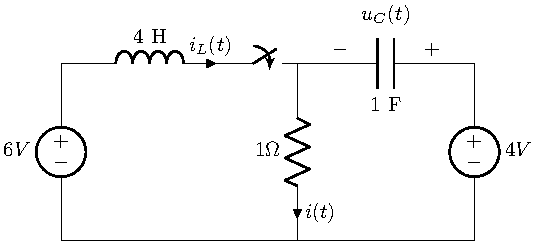
\includegraphics{../figs/ejemplo_2orden.pdf}
%	    \end{figure}
%\end{frame}

%%%%%%%%%%%%%%%

%\begin{frame}
%
%    \vspace{10mm}
%    \begin{center}
%        \LARGE \textcolor{red}{ACTUALIZACIÓN PENDIENTE DE LAS DIAPOSITIVAS}
%    \end{center}
%
%    \vspace{5mm}
%    Falta por añadir:
%    \begin{itemize}
%        \item Circuitos de $2^{\textrm{do}}$ orden
%    \end{itemize}
%\end{frame}

%%%%%%%%%%%%%%%

\begin{frame}{Interludio: \hspace{3mm}temas de investigación en sistemas eléctricos}

    \vspace{7mm}
    \begin{itemize}
        \item Operación económica de sistemas eléctricos nacionales con baja inercia, \href{https://raw.githubusercontent.com/badber/Miscellany/master/Operacion_sistemas_baja_inercia.pdf}{link}
    \end{itemize}

    \vspace{2mm}
    \begin{center}
        \includegraphics[width=.8\linewidth]{../figs/futuristicGrid.jpg}
        % \includegraphics[width=1\linewidth]{../figs/presentGrid_futureGrid.png}
    \end{center}
\end{frame}


\end{document}
